\documentclass[12pt]{report}
\usepackage[paper=letterpaper,margin=3cm]{geometry}
\usepackage{amsmath}
\usepackage{amssymb}
\usepackage{amsfonts}
\usepackage{newtxtext, newtxmath}
\usepackage{enumitem}
\usepackage{titling}
\usepackage{nccmath}
\usepackage[colorlinks=true]{hyperref}
\usepackage[utf8]{inputenc}
\usepackage{graphicx}
\usepackage{tcolorbox}
\usepackage{pgfplots}
\usepackage{listings}
\usepackage{xcolor}

\lstset{
    language=Matlab,
    basicstyle=\ttfamily,
    keywordstyle=\color{blue},
    stringstyle=\color{red},
    commentstyle=\color{green!70!black},
    columns=fullflexible,
    breaklines=true,
    postbreak=\mbox{\textcolor{red}{$\hookrightarrow$}\space},
}

\graphicspath{ {images/} }
\tcbuselibrary{raster}

% Externalising the figures used:
\usepgfplotslibrary{external}
\tikzexternalize

\setlength{\droptitle}{-6em}
\pgfplotsset{width=10cm,compat=1.18}
% Enter the specific assignment number and topic of that assignment below, and replace "Your Name" with your actual name.
\title{Assignment \# 1: MATH1051} 
\author{Jamie Chen\\ \text{Student Number:} \texttt{48093189} \\ \text{Semester 2, 2023}}
\date{\today}

\begin{document}
\maketitle
\begin{enumerate}[leftmargin=\labelsep]
%% Question 1

    \item {\bf (1 mark each)} Determine the domains (as a subset of $\mathbb{R}$) of the functions:
        \begin{enumerate}
            \item  $f_1(x)=\frac{1}{e^x-e^{-x}}$
                \begin{tcolorbox}
                    \begin{itemize}[label={}]
                        \item The domain of this function $f_1(x)$ is $\mathbb{R} \setminus \{0\}$. As the denominator of the function $f_1(x)$ is $e^x-e^{-x}$, we can see that the function is undefined when $e^x-e^{-x}=0$. This occurs when $e^x=e^{-x}$, which is when $x=0$. Therefore, the domain of this function is $\mathbb{R} \setminus \{0\}$.
                    \end{itemize}
                \end{tcolorbox}
            \item  $f_2(x)=\frac{1}{\sqrt{4-x^2}}$
                \begin{tcolorbox}
                    \begin{itemize}[label={}]
                        \item The domain of this function $f_2(x)$ is $(-2,2)$ (non-inclusive). As the denominator of the function $f_2(x)$ is $\sqrt{4-x^2}$, we can see that the function is undefined when $\sqrt{4-x^2}=0$. This occurs when $4-x^2=0$, which is when $x=\pm2$. Therefore, the domain of this function is $(-2,2)$ (non-inclusive).
                    \end{itemize}
                \end{tcolorbox}
            \item  $f_3(x)= \log \arccos x$ 
                \begin{tcolorbox}
                    \begin{itemize}[label={}]
                        \item The domain of this function $f_3(x)$ is $[-1,1)$ (inclusive from the left, exclusive from the right). As the function $f_3(x)$ is a composition of two functions, we must consider the domain of both functions. The domain of the function $\arccos x$ is $[-1,1]$, and the domain of the function $\log x$ is $(0,\infty)$. Therefore, the domain of the function $f_3(x)$ is $[-1,1)$ (inclusive from the left, exclusive from the right). 
                    \end{itemize}
                \end{tcolorbox}
        \end{enumerate}
            
%% New Page
\newpage
%% Question 2  

    \item {\bf (3 marks)} Given is the function $g(x)=x^2+3x$. For a second function $f$ with $f(3)=0$ we find $(g \circ f)(x)=x^2-3x$. What is the function $f$? Is $f$ unique?
        \begin{tcolorbox}
            \begin{itemize}[label={}]
                \item The function $f$ can be a simple linear function, such as $f(x)=x-3$. 
                \begin{equation*}
                    \begin{split}
                        (g \circ f)(x) &= g(f(x)) \\
                        &= (x-3)^2+3(x-3) \\
                        &= x^2-6x+9+3x-9 \\
                        &= x^2-3x
                    \end{split}
                \end{equation*}
                \item We can prove that this function is unique or not by substituting $f(x)=x-3$ into the function $g(x)$ and seeing if it is equal to the function $(g \circ f)(x)$.
                \begin{equation*}
                    \begin{split}
                        g(x) &= x^2+3x \\
                        g(f(x)) &= (x-3)^2+3(x-3) \\
                        &= x^2-6x+9+3x-9 \\
                        &= x^2-3x
                    \end{split}
                \end{equation*}
            \end{itemize}
        \end{tcolorbox}

%% New Page
\newpage        
%% Question 3
    
    \item {\bf (1 mark each)} Determine which of the following functions are 1-1? Prove your answer.
        \begin{enumerate}
            \item $f_1(x)=e^{-x^2}$
                \begin{tcolorbox}
                    \begin{itemize}[label={}]
                        \item Defined in the workbook:
                        \begin{quote}
                            A function $f: X\to Y$ is called {\bf one-to-one} (or {\bf injective}) if $\forall x_1,x_2 \in \mathbb{R} \cap X$, $f(x_1)=f(x_2)$ $\implies$ $x_1=x_2$.
                        \end{quote}
                        \item
                        \item The function $f_1(x)=e^{-x^2}$ is not one-to-one as it is not a strictly decreasing function or strictly increasing function. Additionally, if we follow the definition of a one-to-one function:
                        \begin{equation*}
                            \begin{split}
                                f_1(x_1) &= f_1(x_2) \\
                                e^{-x_1^2} &= e^{-x_2^2} \\
                                \ln e^{-x_1^2} &= \ln e^{-x_2^2} \\
                                -x_1^2 &= -x_2^2 \\
                                x_1^2 &= x_2^2 \\
                                x_1 &= \pm x_2
                            \end{split}
                        \end{equation*}
                        \item Therefore, the function $f_1(x)=e^{-x^2}$ is not one-to-one.
                        
                    \end{itemize}
                \end{tcolorbox}
                
\newpage
            \item $f_2(x)=2x^2-3x+1$
                \begin{tcolorbox}
                    \begin{itemize}[label={}]
                        \item The function $f_2(x)=2x^2-3x+1$ is not one-to-one. There are several reasons for this:
                        \begin{enumerate}
                            \item[1.] The function $f_2(x)$ is not strictly increasing or decreasing.
                            \item[2.] The function $f_2(x)$ is a quadratic function, and therefore can have two values of $x$ that correspond to the same value of $y$. 
                            \item[3.] Using the definition of a one-to-one function:
                            \begin{equation*}
                                f_1(x_1) = f_1(x_2) \implies x_1 = x_2 \\
                            \end{equation*} 
                            \begin{equation*}
                                2x_1^2-3x_1+1 = 2x_2^2-3x_2+1 \implies x_1 = x_2
                            \end{equation*}
                            \item[] We can see that the function $f_2(x)$ is not one-to-one as there are multiple values of $x$ that correspond to the same value of $y$.
                            \begin{center}
                                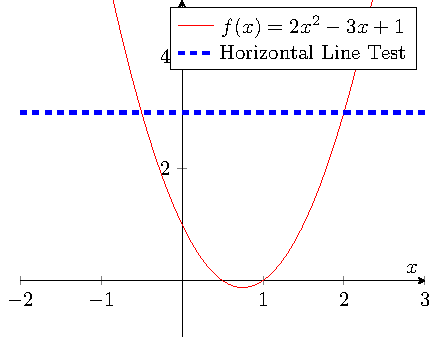
\includegraphics[width=0.8\linewidth]{lib/figures/Figure1.pdf}
                            \end{center}
                        \end{enumerate}
                    \end{itemize}
                \end{tcolorbox}

\newpage
            \item $f_3(x)=|x|+2 \cdot x$
                \begin{tcolorbox}
                    \begin{itemize}[label={}]
                        \item The function $f_3(x)=|x|+2 \cdot x$ is one-to-one. There are several reasons for this (using the definition of a one-to-one function):
                        \begin{equation*}
                            \begin{array}{r@{~=~}l}
                                f_3(x_1) & f_3(x_2) \\ [2ex]
                                |x_1|+2 \cdot x_1 & |x_2|+2 \cdot x_2 \\ [2ex]
                            \end{array}
                        \end{equation*}
                        \item There are four cases that we need to consider:
                        \item The first case is when $x_1,x_2 < 0$, the second case is when $x_1,x_2 \geq 0$, the third case is when $x_1 < 0$ and $x_2 \geq 0$, and the fourth case is when $x_1 \geq 0$ and $x_2 < 0$.
                        \item There are two cases in which that they are arbitrary, and two cases in which they are not arbitrary. 
                        \item The two cases in which they are arbitrary are the third and fourth cases.
                        \item In this case, lets consider that there are two cases:
                        \item The first case is when $x_1,x_2 \geq 0$:
                        \item In this case, we can assume that $|x_1|=x_1$ and $|x_2|=x_2$. We can then determine the equation for this case:
                    \end{itemize}
                \end{tcolorbox}
                \begin{tcolorbox}
                    \begin{itemize}[label={}]
                        \item
                        \begin{equation*}
                            |x_1|+2 \cdot x_1 = |x_2|+2 \cdot x_2
                        \end{equation*}
                        \item Simplifying this equation gives us:
                        \begin{equation*}
                            3x_1 = 3x_2
                        \end{equation*}
                        \item Dividing both sides by 3 gives us:
                        \begin{equation*}
                            x_1 = x_2
                        \end{equation*}
                        \item We can now determine the second case.
                        \item The second case is when $x_1,x_2 < 0$:
                        \item In this case, we can assume that $|x_1|=-x_1$ and $|x_2|=-x_2$. We can then determine the equation for this case:
                        \begin{equation*}
                            -x_1+2 \cdot x_1 = -x_2+2 \cdot x_2
                        \end{equation*}
                        \item Simplifying this equation gives us:
                        \begin{equation*}
                            x_1 = x_2
                        \end{equation*}
                        \item After determining both cases for the absolute value function, we can see that the function $f_3(x)=|x|+2 \cdot x$ is one-to-one.
                    \end{itemize}
                \end{tcolorbox}
        \end{enumerate}
            
%% New Page
\newpage
%% Question 4 

    \item {\bf (1 mark each)} Determine what the following limits are or show that they do not exist.
        \begin{enumerate}
            \item $ {\lim \limits_{{n\rightarrow \infty}}} \frac{(n^2+4 n-27)(n^3-1)}{(n(n-1))^2} $
                \begin{tcolorbox}
                    \begin{itemize}[label={}]
                        \item We can determine the limit of this function by using the following steps:
                        \item We can first expand the numerator and denominator of the function and then divide each term by the highest power of $n$ in the denominator:
                    \end{itemize}
                    \begin{equation*}
                        \begin{array}{r@{~=~}l}
                            {\lim \limits_{{n\rightarrow \infty}}} \frac{(n^2+4 n-27)(n^3-1)}{(n(n-1))^2} & {\lim \limits_{{n\rightarrow \infty}}} \frac{n^5+4n^4-27n^3-n^3+1}{n^4-2n^3+n^2} \\ [2ex]
                            & {\lim \limits_{{n\rightarrow \infty}}} \frac{n^5+4n^4-28n^3+1}{n^4-2n^3+n^2} \\ [2ex]
                            & {\lim \limits_{{n\rightarrow \infty}}} \frac{n+4-\frac{28}{n}+\frac{1}{n^3}}{1-\frac{2}{n}+\frac{1}{n^2}} \\ [2ex]
                            & \frac{\infty}{1} \\ [2ex]
                            & \infty
                        \end{array}
                    \end{equation*}
                    Therefore the limit does not exist when $n \rightarrow \infty$ as the limit is $\infty$.
                \end{tcolorbox}
            \item $\lim \limits_{n\rightarrow \infty} \frac{3n^2-9n + 48}{4n^3}$
                \begin{tcolorbox}
                    \begin{itemize}[label={}]
                        \item We can determine the limit for this function by using the same steps as the previous question.
                        \item We can divide each term by $n^2$ in the denominator.
                        \item As $n \rightarrow \infty$, $\frac{1}{n^2} \rightarrow 0$. Therefore the term will approach 0.
                        \item 
                    \end{itemize}
                    \begin{equation*}
                        \begin{array}{r@{~=~}l}
                            {\lim \limits_{{n\rightarrow \infty}}} \frac{3n^2-9n + 48}{4n^3} & {\lim \limits_{{n\rightarrow \infty}}} \frac{3-\frac{9}{n} + \frac{48}{n^2}}{4n} \\ [2ex]
                            & {\lim \limits_{{n\rightarrow \infty}}} \frac{3}{4n} - \frac{9}{4n^2} + \frac{12}{n^3} \\ [2ex]
                            & 0 \quad \text{Since the limit of } \frac{1}{n} = 0 \text{ as } n \rightarrow \infty.
                        \end{array}
                    \end{equation*}
                    \begin{itemize}[label={}]
                        \item
                        \item Therefore the limit of the function is 0.
                        \item \item
                    \end{itemize}
                \end{tcolorbox}
            \item $\lim \limits_{n\rightarrow \infty} \frac{(3n+1)^3-27n^3}{n^2}$
                \begin{tcolorbox}
                    \begin{itemize}[label={}]
                        \item Similar to part (a), we can determine the limit of this function by using the following steps:
                        \item We can first expand the numerator and denominator of the function and then divide each term by the highest power of $n$ in the denominator.
                        \item As $\frac{1}{n} \rightarrow 0$ and $\frac{1}{n^2} \rightarrow 0$ as $n \rightarrow \infty$, we can ignore these terms as they will eventually approach 0.
                    \end{itemize}
                    \begin{equation*}
                        \begin{array}{r@{~=~}l}
                            {\lim \limits_{{n\rightarrow \infty}}} \frac{(3n+1)^3-27n^3}{n^2} & {\lim \limits_{{n\rightarrow \infty}}} \frac{27n^3+27n^2+9n+1-27n^3}{n^2} \\ [2ex]
                            & {\lim \limits_{{n\rightarrow \infty}}} \frac{27n^2+9n+1}{n^2} \\ [2ex]
                            & {\lim \limits_{{n\rightarrow \infty}}} (27+\frac{9}{n}+\frac{1}{n^2}) \\ [2ex]
                            & 27
                        \end{array}
                    \end{equation*}
                    \begin{itemize}[label={}]
                        \item $\therefore$ The limit is 27 as $n \rightarrow \infty$.
                    \end{itemize}
                \end{tcolorbox}
\newpage
            \item $\lim \limits_{n\rightarrow \infty} \frac{2n^2}{2n-1}-n$
                \begin{tcolorbox}
                    \begin{itemize}[label={}]
                        \item To determine this limit, we can use similar steps as the previous question in part (a).
                        \item We can divide each term in the numerator by the highest power of $n$ in the denominator.
                        \item As $\frac{1}{n} \rightarrow 0$ as $n \rightarrow \infty$, we can ignore this term as it will eventually approach 0.
                    \end{itemize}
                    \begin{equation*}
                        \begin{array}{r@{~=~}l}
                            {\lim \limits_{{n\rightarrow \infty}}} \frac{2n^2}{2n-1}-n & {\lim \limits_{{n\rightarrow \infty}}} \frac{2n^2}{2n-1}-\frac{n(2n-1)}{2n-1} \\ [2ex]
                            & {\lim \limits_{{n\rightarrow \infty}}} \frac{2n^2-n(2n-1)}{2n-1} \\ [2ex]
                            & {\lim \limits_{{n\rightarrow \infty}}} \frac{2n^2-2n^2+n}{2n-1} \\ [2ex]
                            & {\lim \limits_{{n\rightarrow \infty}}} \frac{n}{2n-1} \\ [2ex]
                            & {\lim \limits_{{n\rightarrow \infty}}} \frac{1}{2-\frac{1}{n}} \\ [2ex]
                            & \mfrac{1}{2} \quad \text{Since the limit of } \frac{1}{n} = 0 \text{ as } n \rightarrow \infty.
                        \end{array}
                    \end{equation*}
                    \begin{itemize}[label={}]
                        \item Therefore, the limit is $\frac{1}{2}$ as $n \rightarrow \infty$.
                    \end{itemize}
                \end{tcolorbox}
\newpage
            \item $\lim \limits_{n\rightarrow \infty} \sqrt{n(n+1)}-n$
                \begin{tcolorbox}
                    \begin{itemize}[label={}]
                        \item In this limit, we can find the limit by rationalising the numerator.
                        \item To do this we can multiply the numerator and denominator by the conjugate of the numerator:
                        \begin{equation*}
                            \begin{array}{r@{~=~}l}
                                {\lim \limits_{{n\rightarrow \infty}}} \sqrt{n(n+1)}-n & {\lim \limits_{{n\rightarrow \infty}}} \sqrt{n(n+1)}-n \times \frac{\sqrt{n(n+1)}+n}{\sqrt{n(n+1)}+n} \\ [2ex]
                                & {\lim \limits_{{n\rightarrow \infty}}} \frac{n(n+1)-n^2}{\sqrt{n(n+1)}+n} \\ [2ex]
                            \end{array}
                        \end{equation*}
                        \item We can then simplify the equation to find the limit:
                        \begin{equation*}
                            \begin{array}{r@{~=~}l}
                                & {\lim \limits_{{n\rightarrow \infty}}} \frac{n^2+n-n^2}{\sqrt{n(n+1)}+n} \\ [2ex]
                                & {\lim \limits_{{n\rightarrow \infty}}} \frac{n}{\sqrt{n(n+1)}+n} \\ [2ex]
                                & {\lim \limits_{{n\rightarrow \infty}}} \frac{1}{\sqrt{1+\frac{1}{n}}+1} \\ [2ex]
                                & \frac{1}{2} \quad \text{Since the limit of } \frac{1}{n} = 0 \text{ as } n \rightarrow \infty.
                            \end{array}
                        \end{equation*}
                    \end{itemize}
                \end{tcolorbox}
        \end{enumerate}

%% New Page
\newpage
%% Question 5

    \item {\bf (1 mark each)} Consider the sequence $a_n$ defined by the recursion
        \begin{equation}
            a_n=a_{n-1}-\frac{1}{4}a_{n-2}
        \end{equation} for $n=3,4,5,\dots$.
        \begin{enumerate}
            \item Calculate $h$ such that $a_n=h^{n-1}$ fulfils the recursive definition.
                \begin{tcolorbox}
                    \begin{itemize}[label={}]
                        \item To calculate $h$ we can substitute $a_n=h^{n-1}$ into the recursive definition:
                        \begin{equation*}
                            h^{n-1}=h^{n-2}-\frac{1}{4}h^{n-3}
                        \end{equation*}
                        \item We can now divide both sides by $h^{n-3}$:
                        \begin{equation*}
                            h^2=h- \frac{1}{4}
                        \end{equation*}
                        \item Solving h in terms of the quadratic formula:
                        \begin{equation*}
                            h=\frac{-(-1) \pm \sqrt{1-4 \cdot 1 \cdot \frac{1}{4}}}{2 \cdot 1}
                        \end{equation*}
                        \begin{equation*}
                            h=\frac{1 \pm \sqrt{1-1}}{2}
                        \end{equation*}
                        \begin{equation*}
                            h=\frac{1 \pm 0}{2}
                        \end{equation*}
                        \begin{equation*}
                            \therefore h=\frac{1}{2}
                        \end{equation*}
                    \end{itemize}
                \end{tcolorbox}
\newpage 
            \item What is the limit of the sequence $a_n$ (if it exists)?
                \begin{tcolorbox}
                    \begin{itemize}[label={}]
                        \item To find the limit of the sequence $a_n$ we can start by looking at the recursive definition.
                        \item Since $a_n = a_{n-1} - \frac{1}{4}a_{n-2}$, we can tell that the sequence is dependent on two previous terms; $a_{n-1}$ and $a_{n-2}$.
                        \item Because of this, the limit when $n$ approaches infinity will be dependent on the previous two terms.
                        \item Since the previous terms will always be smaller than the current term and that the terms will get infinitely smaller, the limit of the sequence $a_n$ will be 0.
                    \end{itemize}
                    \begin{itemize}[label={}]
                        \item We can also prove this by using the limit definition:
                        \item We can assume that there is a limit $L$ such that:
                        \begin{equation*}
                            \lim \limits_{n\rightarrow \infty} a_n = L
                        \end{equation*}
                        \item Since the sequence is defined recursively, we can substitute $L$ into the recursive definition:
                        \begin{equation*}
                            L=L-\frac{1}{4}L
                        \end{equation*}
                        \item We can then simplify the equation to find the limit:
                        \begin{equation*}
                            L=0
                        \end{equation*}
                        \item Therefore, if the limit exists for the sequence, the limit of the sequence $a_n$ is 0.
                    \end{itemize}
                \end{tcolorbox}
        \end{enumerate}

%% New Page
\newpage
%% Question 6

    \item {\bf (1 mark each)} Given is the sequence $b_n$ defined in recursive form
        \begin{equation*}
            b_n=\frac{1}{2}\left(b_{n-1}+\frac{A}{b_{n-1}} \right)
        \end{equation*} for a given $A>0$. You can assume that all values of $b_n$ are non-zero.
        \begin{enumerate}
            \item For $A=2$ use your calculator (or MATLAB) to calculate the first four values of the sequence $b_n$ starting from $b_1=A$ (this is for $n=1,2,3,4$). Inspecting these values do you expect the sequence to be convergent or to be divergent?
                \begin{tcolorbox}
                    \begin{itemize}[label={}]
                        \item Given that A $>$ 0, I expect the sequence to be convergent. This is because as n increases, the value of $b_n$ will approach the limit of the sequence.
                        \item Substituting $n=1,2,3,4$ into the recursive definition:
                        \begin{equation*}
                            \begin{array}{r@{~=~}l}
                                b_{1} & A \\ [2ex]
                                b_{2} & \frac{1}{2}\left(b_{1}+\frac{A}{b_{1}} \right) \\ [2ex]
                                & \frac{1}{2}\left(A+\frac{A}{A} \right) \\ [2ex]
                                & \frac{1}{2}\left(A+1 \right) \\ [2ex]
                                & \frac{A+1}{2} \\ [2ex]
                                & \frac{A}{2}+\frac{1}{2} \\ [2ex]
                            \end{array}
                            \begin{array}{r@{~=~}l}
                                b_{3} & \frac{1}{2}\left(b_{2}+\frac{A}{b_{2}} \right) \\ [2ex]
                                & \frac{1}{2}\left(\frac{A}{2}+\frac{1}{2}+\frac{A}{\frac{A}{2}+\frac{1}{2}} \right) \\ [2ex]
                                & \frac{A^2+6A+1}{4A+4} \\ [2ex]
                                b_{4} & \frac{1}{2}\left(b_{3}+\frac{A}{b_{3}} \right) \\ [2ex]
                                & \frac{1}{2}\left(\frac{A^2+6A+1}{4A+4}+\frac{A}{\frac{A^2+6A+1}{4A+4}} \right) \\ [2ex]
                                
                            \end{array}
                        \end{equation*}
                        \item We can then substitute $A=2$ into the recursive definition:
                        \begin{equation*}
                            \begin{array}{r@{~=~}l}
                                b_{1} & 2 \\ [2ex]
                                b_{2} & \frac{2}{2}+\frac{1}{2} \\ [2ex]
                                b_{2} & \frac{3}{2} \\ [2ex]
                            \end{array}
                            \begin{array}{r@{~=~}l}
                                b_{3} & \frac{1}{2}\left(\frac{2}{2}+\frac{1}{2}+\frac{2}{\frac{2}{2}+\frac{1}{2}} \right) \\ [2ex]
                                b_{3} & \frac{17}{12} \\ [2ex]
                                b_{4} & \frac{1}{2}\left(\frac{17}{12}+\frac{2}{\frac{17}{12}} \right) \\ [2ex]
                                b_{4} & \frac{577}{408} \\ [2ex]
                            \end{array}
                        \end{equation*}
                    \end{itemize}
                \end{tcolorbox}
\newpage
            \item Assume you know the sequence $b_n$ is converging, what would be its limit (or its limits)? Justify your answer. Is it consistent with your result of part (a)?
                \begin{tcolorbox}
                    \begin{itemize}[label={}]
                        \item We can show this by using the recursive definition:
                        \item Because the sequence is increasing and bounded above, we can find the limit and equality of the sequence by solving the equation:
                        \item Let $L$ be the limit of the sequence $b_n$:
                        \begin{equation*}
                            L=\frac{1}{2}\left(L+\frac{A}{L} \right)
                        \end{equation*}
                        \item Multiplying both sides by 2:
                        \begin{equation*}
                            2L=L+\frac{A}{L}
                        \end{equation*}
                        \item Subtracting $L$ from both sides:
                        \begin{equation*}
                            L=\frac{A}{L}
                        \end{equation*}
                        \item Multiplying both sides by $L$:
                        \begin{equation*}
                            L^2=A
                        \end{equation*}
                        \item Taking the square root of both sides:
                        \begin{equation*}
                            L=\pm \sqrt{A}
                        \end{equation*}
                        \item Since $A>0$, we know that the Limit will be at $L=\sqrt{A}$.
                        \item Since we know that $A=2$, we can substitute this into the equation:
                        \begin{equation*}
                            L=\sqrt{2}
                        \end{equation*}
                        \item Therefore, the limit of the sequence $b_n$ is $\sqrt{2}$.
                    \end{itemize}
                \end{tcolorbox}
        \end{enumerate}

%% New Page
\newpage
%% Question 7

    \item {\bf (1 mark each)} Assume you have given a sequence $c_n$ with non-zero values ($c_n\neq0$ for $n=1,2,\dots$) that fulfils the condition
        \begin{equation}
            \left|\frac{c_n}{c_{n-1}}\right|\leq q
        \end{equation} for all $n=1,2,3,\dots$ for some fixed constant q with $0<q<1$.
        \begin{enumerate}
            \item Show that $c_n\to0$ for $n\to \infty$. (Hint: use the squeeze theorem)
                \begin{tcolorbox}
                    \begin{itemize}[label={}]
                        \item To show that the sequence $c_n$ converges to 0, we can use the squeeze theorem. We can start by rearranging the inequality:
                        \begin{equation*}
                            |c_n| \leq q|c_n-1|
                        \end{equation*}
                        \item Since we know that $0<q<1$, the absolute value of $c_n$ will always be less than the absolute value of $c_{n-1}$. This means that the sequence $c_n$ will always be squeezed between 0 and $q|c_n-1|$. Since $q|c_n-1|$ converges to 0, the sequence $c_n$ must also converge to 0. We can show this by using the squeeze theorem:
                        \begin{equation*}
                            |c_n| \leq q^n|c_{n-1}|
                        \end{equation*}
                        \item Since $q^n|c_{n-1}|$ converges to 0, the sequence $c_n$ must also converge to 0.
                        \item Therefore the sequnce $c_n$ converges to 0 when $n\to \infty$.
                    \end{itemize}
                \end{tcolorbox}
\newpage
            \item Use the result from part(a) to show that $\displaystyle{\lim_{n \to \infty}}\,\,\, \frac{2^n}{n!}=0$.
                \begin{tcolorbox}
                    \begin{itemize}[label={}]
                        \item Using the result from Part A, we can show that the $\displaystyle{\lim_{n \to \infty}}\,\,\, \frac{2^n}{n!}=0$.
                        \item We can start by defining a new sequence $a_n$:
                        \begin{equation*}
                            a_n = \frac{2^n}{n!} \quad \text{ for } n=1,2,3,\dots
                        \end{equation*}
                        \item We then divide the sequence $a_n$ by $a_{n-1}$:
                        \begin{equation*} \frac{a_n}{a_{n-1}} = \frac{\frac{2^n}{n!}}{\frac{2^{n-1}}{(n-1)!}}
                        \end{equation*}
                        \item We can then simplify the equation:
                        \begin{equation*}
                           = \frac{2^n}{n!} \times \frac{(n-1)!}{2^{n-1}}
                        \end{equation*}
                        \item We can then cancel out the $2^{n-1}$ and $(n-1)!$:
                        \begin{equation*}
                            = \frac{2^n}{n \times (n-1)!} \times \frac{(n-1)!}{2^{n-1}}
                        \end{equation*}
                        \begin{equation*}
                            =\frac{2^n}{n} \times \frac{1}{2^{n-1}}
                        \end{equation*}
                        \item We can then simplify the equation:
                        \begin{equation*}
                            =\frac{2 \times 2^{n-1}}{n} \times \frac{1}{2^{n-1}}
                        \end{equation*}
                        \item We can now cancel out the $2^{n-1}$:
                        \begin{equation*}
                            =\frac{2}{n}
                        \end{equation*}
                        \item Since $\frac{2}{n} \leq 1$ for all $n \geq 3$, we can apply the result from part A to show that the sequence $a_n$ converges to 0 as $n$ approaches infinity.
                    \end{itemize}
                \end{tcolorbox}
\newpage
            \item Again: use the result from part(a) to show that $\displaystyle{\lim_{n \to \infty}}\,\,\, \frac{1}{3^nn^3}=0$.
                    \begin{tcolorbox}
                        \begin{itemize}[label={}]
                            \item Similar to Part B, we can use the result from Part A to show that the $\displaystyle{\lim_{n \to \infty}}\,\,\, \frac{1}{3^nn^3}=0$.
                            \item We can start by defining a new sequence $b_n$:
                            \begin{equation*}
                                b_n = \frac{1}{3^nn^3} \quad \text{ for } n=1,2,3,\dots
                            \end{equation*}
                            \item We then divide the sequence $b_n$ by $b_{n-1}$:
                            \begin{equation*} \frac{b_n}{b_{n-1}} = \frac{\frac{1}{3^nn^3}}{\frac{1}{3^{n-1}(n-1)^3}} 
                            \end{equation*}
                            \item Simplify by reciprocating the denominator and multiplying by the numerator:
                            \begin{equation*}
                                = \frac{1}{3^nn^3} \times \frac{3^{n-1}(n-1)^3}{1}
                            \end{equation*}
                            \item Simplify further:
                            \begin{equation*}
                               \frac{1}{n^3} \times \frac{(n-1)^3}{1} = \frac{(n-1)^3}{3n^3} = \frac{n^3-3n^2+3n-1}{3n^3} 
                            \end{equation*}
                            \item We can then divide the numerator and denominator by $n^3$:
                            \begin{equation*}
                                = \frac{1}{3} - \frac{1}{n} + \frac{1}{n^2} - \frac{1}{n^3}
                            \end{equation*}
                            \item We now determine this limit:
                            \begin{equation*}
                                {\lim_{n \to \infty}}\,\,\, \frac{1}{3} - \frac{1}{n} + \frac{1}{n^2} - \frac{1}{n^3} = \frac{1}{3} - 0 + 0 - 0 = \frac{1}{3}
                            \end{equation*}
                            \item Since $\frac{1}{3} \leq 1$ for all $n \geq 2$, we can apply the result from part A to show that the sequence $b_n$ converges to $\frac{1}{3}$ as $n$ approaches infinity.
                        \end{itemize}
                    \end{tcolorbox}
        \end{enumerate} 


\end{enumerate}
\end{document}